
%	\Mati{Explicar que las innovaciones no dan tan bien}
%	\Mati{La matriz de rotación no la estima tan bien}
%	\Mati{El sesgo mantiene la tendencia pero no llega al valor}
%	\Mati{Lo demás lo estima razonablemente bien}
Se realiza la discretización de primer orden ($e^{At}\approx I + AT$) de la matriz $A(t)$ de la Ecuación \eqref{eq:matrix_cont}:
		\begin{equation*}
			A_d = \begin{bmatrix}	1& 0& T& 0&           0&           0&           0&           0      \\[0.3em]
						0& 1& 0& T&           0&           0&           0&           0      \\[0.3em]
						0& 0& 1& 0& T\,a_x& T\,a_y&           0&           0 \\[0.3em]
						0& 0& 0& 1&           0&           0& T\,a_x& T\,a_y\\[0.3em]
						0& 0& 0& 0&           1&         T\,\omega&           0&           0\\[0.3em]
						0& 0& 0& 0&        -T\,\omega&           1&           0&           0\\[0.3em]
						0& 0& 0& 0&           0&           0&           1&         T\,\omega\\[0.3em]
						0& 0& 0& 0&           0&           0&        -T\,\omega&           1
			\end{bmatrix}
		\end{equation*}
	
		A dicha matriz se la extiende para agregar los sesgos como variables de estado. Como se supone que los sesgos son constantes a lo largo de la tiempo, su dinámica es constante representado como una matriz identidad. Así se obtiene la nueva $A_d$ y $\vect{x}$ como:
		\begin{equation*}
			A_d = \begin{bmatrix}	1& 0& T& 0&           0&           0&           0&           0&      0&      0\\[0.3em]
						0& 1& 0& T&           0&           0&           0&           0&      0&	     0\\[0.3em]
						0& 0& 1& 0& T\,(a_x - b_x)& T\,(a_y - b_y)&           0&           0& 0& 0\\[0.3em]
						0& 0& 0& 1&           0&           0& T\,(a_x - b_x)& T\,(a_y - b_y)& 0& 0\\[0.3em]
						0& 0& 0& 0&           1&         T\,\omega&           0&           0&      0&      0\\[0.3em]
						0& 0& 0& 0&        -T\,\omega&           1&           0&           0&      0&      0\\[0.3em]
						0& 0& 0& 0&           0&           0&           1&         T\,\omega&      0&      0\\[0.3em]
						0& 0& 0& 0&           0&           0&        -T\,\omega&           1&      0&      0\\[0.3em]
						0& 0& 0& 0&           0&           0&           0&           0&      1&      0\\[0.3em]
						0& 0& 0& 0&           0&           0&           0&           0&      0&      1
			\end{bmatrix}\qquad%
			\vect{x} = \begin{bmatrix} {p_x} \\[0.3em] p_y \\[0.3em] {v_x} \\[0.3em] v_y \\[0.3em] c_{11} \\[0.3em] c_{12} \\[0.3em] c_{21} \\[0.3em] c_{22} \\[0.3em] b_x \\[0.3em] b_y \end{bmatrix}
		\end{equation*}

		El siguiente paso es linealizar $A_d$. Para ello se realiza el producto $A_d\,\vect{x}$ obteniendose un vector columna de funciones alineales (producto de estados). Luego se le calcula el jacobiano y se obtiene la matriz linealizada $A^l_d$:
		\begin{equation*}
			A^l_d = \begin{bmatrix}	1& 0& T& 0&           0&           0&           0&           0&      0&      0\\[0.3em]
						0& 1& 0& T&           0&           0&           0&           0&      0&	     0\\[0.3em]
						0& 0& 1& 0& T\,(a_x - b_x)& T\,(a_y - b_y)&           0&           0& -T\,c_{11}& -T\,c_{12}\\[0.3em]
						0& 0& 0& 1&           0&           0& T\,(a_x - b_x)& T\,(a_y - b_y)& -T\,c_{21}& -T\,c_{22}\\[0.3em]
						0& 0& 0& 0&           1&         T\,\omega&           0&           0&      0&      0\\[0.3em]
						0& 0& 0& 0&        -T\,\omega&           1&           0&           0&      0&      0\\[0.3em]
						0& 0& 0& 0&           0&           0&           1&         T\,\omega&      0&      0\\[0.3em]
						0& 0& 0& 0&           0&           0&        -T\,\omega&           1&      0&      0\\[0.3em]
						0& 0& 0& 0&           0&           0&           0&           0&      1&      0\\[0.3em]
						0& 0& 0& 0&           0&           0&           0&           0&      0&      1
			\end{bmatrix}
		\end{equation*}

		En la implementación del algoritmo, cada ciclo genera la matriz $A^l_d = \frac{\partial{f_d}}{\partial \vect{x}}\left| _{\vect{x}=\vect{x}_{k-1/k-1}}\right. $ y a partir de la misma se realiza la predicción y/o corrección del filtro de Kalman tradicional.\\

		\pagebreak
		\indent En la Figura \ref{fig:ej7} se ve la estimación de la trayectoria y no difiere mucho de la trayectoria real. Asimismo, analizando la Figura \ref{fig:7pos} se ve que la posición la sigue con un error muy bajo. Sin embargo, analizando las innovaciones en la Figura \ref{fig:7covinn} se encuentra que la correlación para $v_y$ no es una función ruidosa como en los casos anteriores. Además, por inspección de la Figura \ref{fig:7vel} se halla que la velocidad tarda en converger y cuando lo hace, tiene oscilaciones en los valores de velocidad real constantes. A su vez, los coeficientes de la matriz de rotación $C_{be}$ (Figura \ref{fig:7theta}) tienen una convergencia muy lenta a los valores reales en comparación a los ejercicios anteriores, pero terminan ajustandose. Lo más preocupante es que el filtro de Kalman extendido no puede estimar los sesgos correctamente como se ve en la Figura \ref{fig:7sesgo}. En la simulación se planteó $b_x = \SI{0.2}{\metre\per\second\squared}$ y $b_y=\SI{-.2}{\metre\per\second\squared}$, y el filtro tuvo una tendencia a converger a dichos valores pero no los alcanza a estimar perfectamente.\\
\begin{figure}[H]
\centering
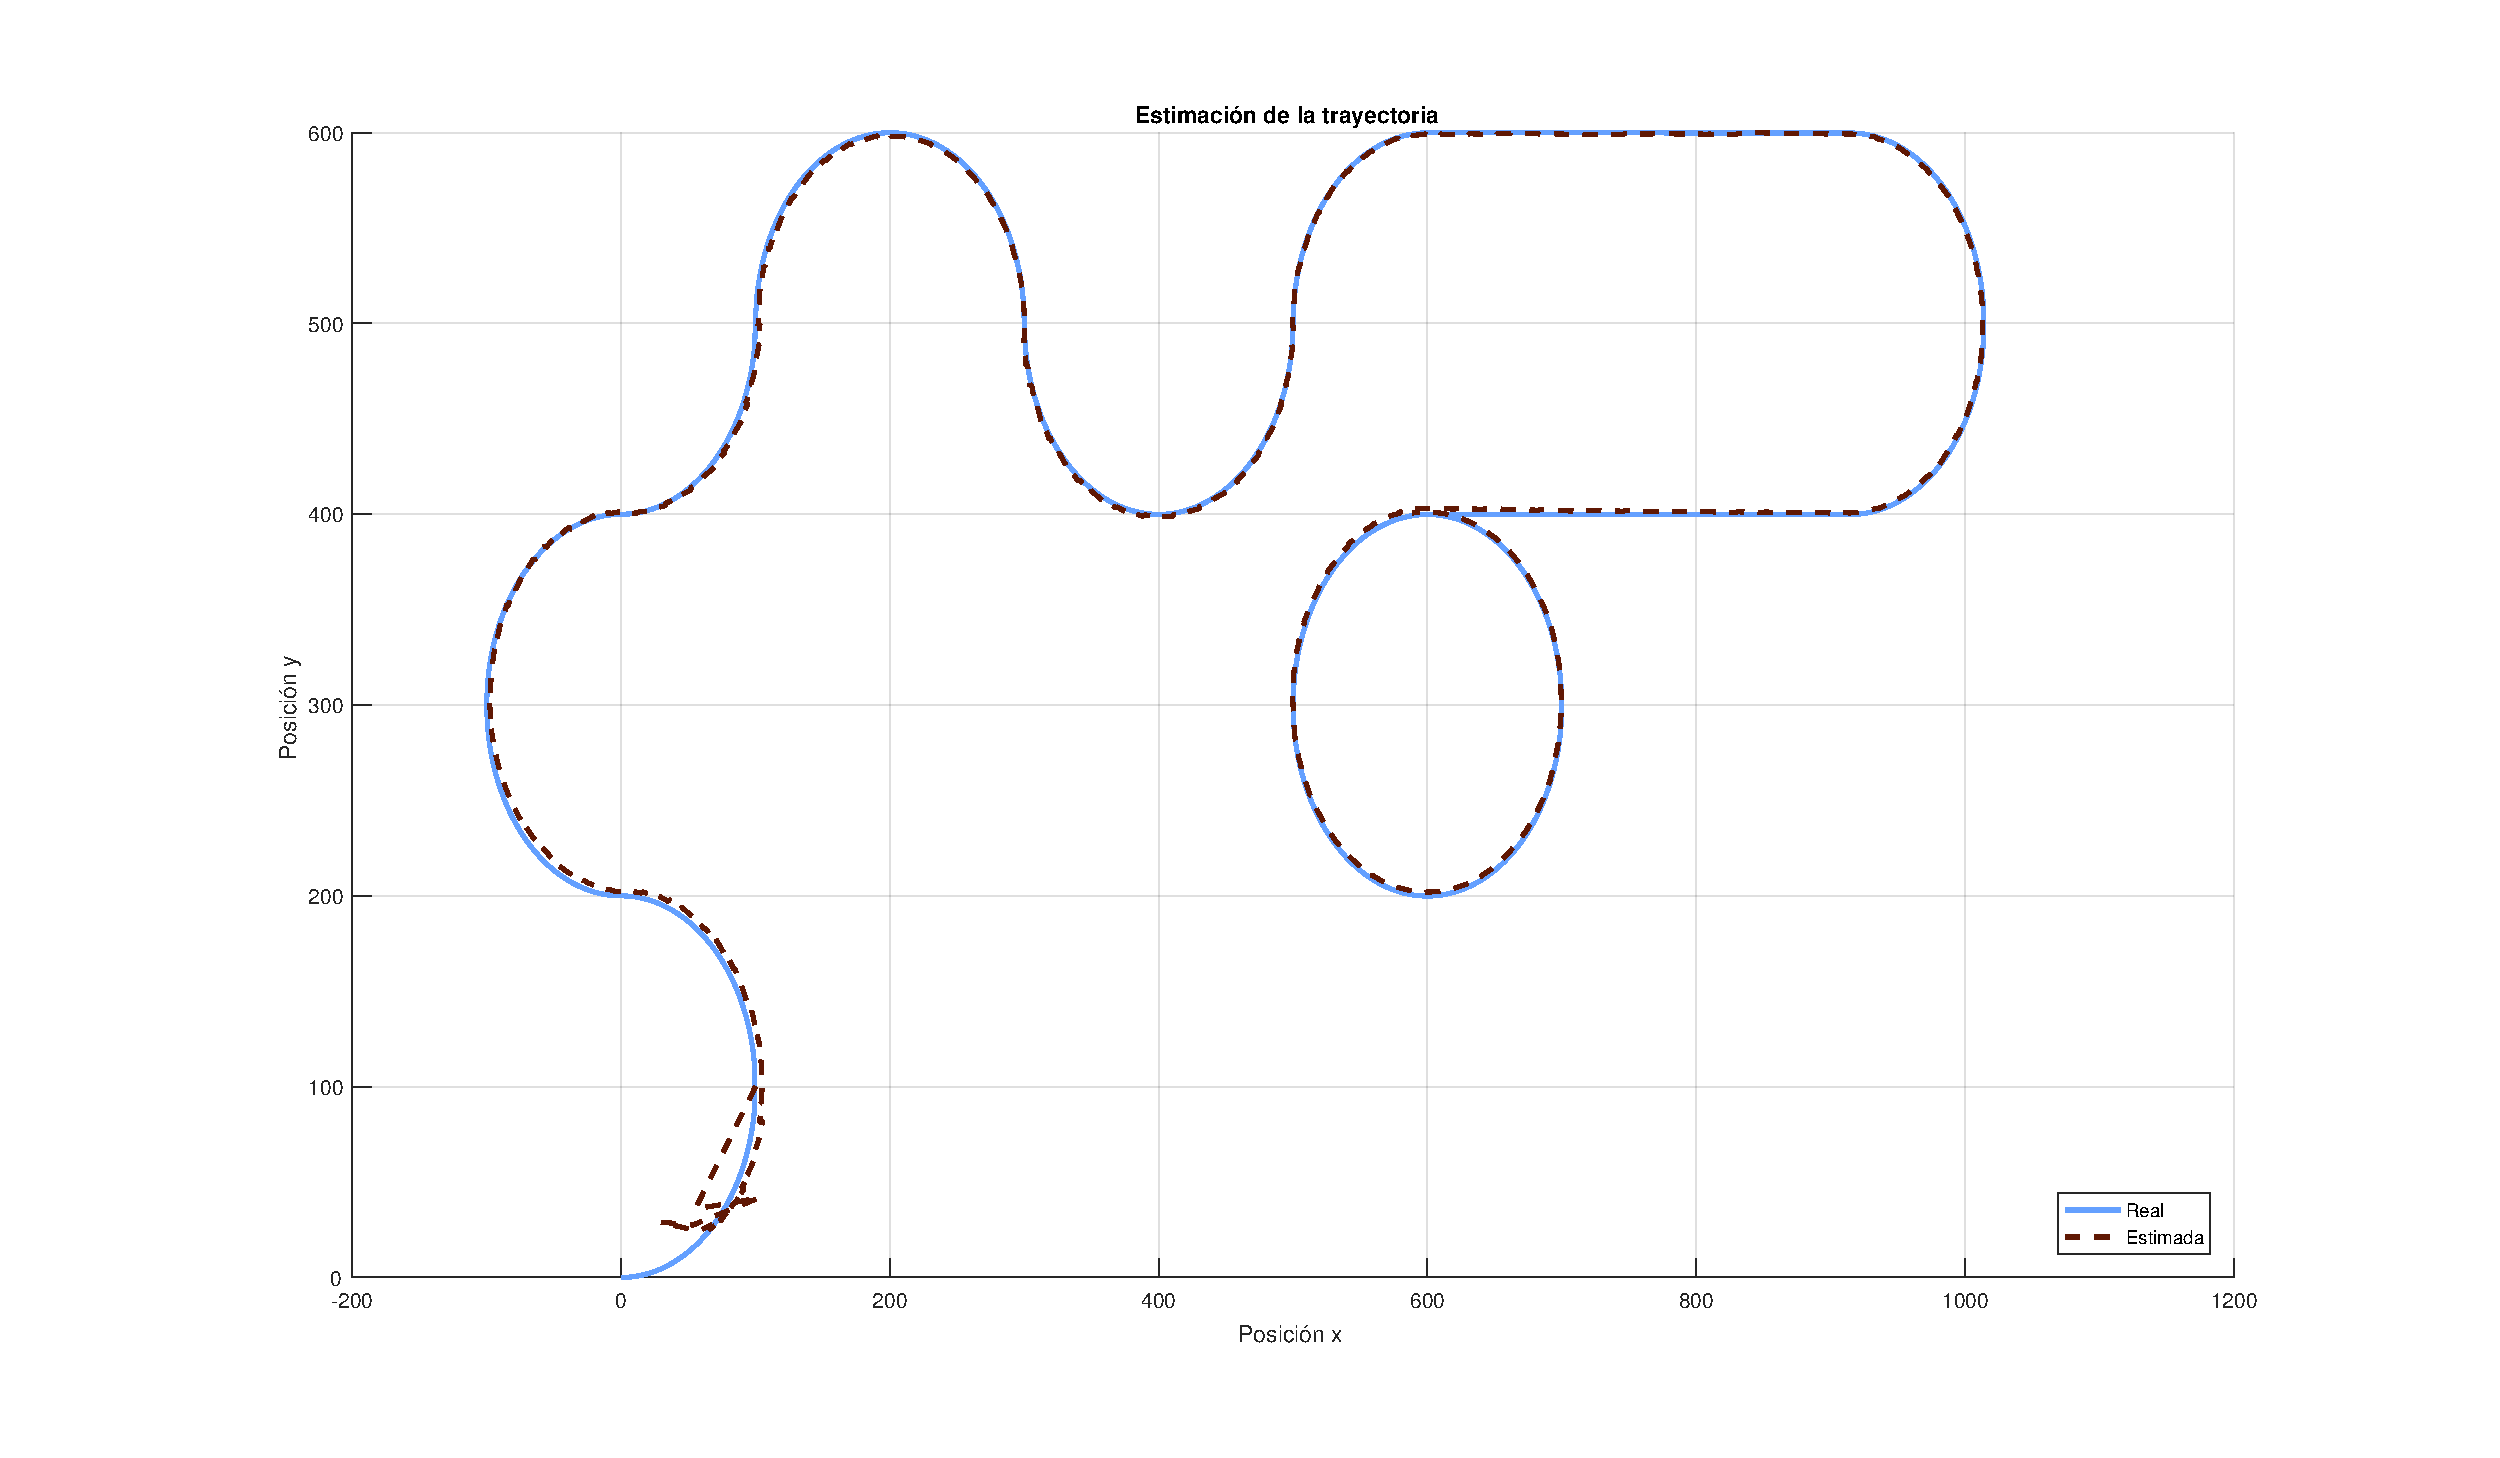
\includegraphics[width=0.9\textwidth, trim= 2cm 2cm 2cm 2cm]{graf_ej7.pdf}
\caption{Estimación de la trayectoria.}
\label{fig:ej7} 
\end{figure}

		\indent Se supone que las irregularidades en las correlaciones de las innovaciones, la lenta convergencia de la velocidad y coeficientes de $C_{be}$ y la imposiblidad de estimar el sesgo están relacionadas. Se revisaron los cálculos de la discretización y linealización de $A$; se utilizaron discretizaciones de primer y segundo orden; se variaron los sesgos a estimar y aún así no se pudieron modificar los problemas enunciados. Una hipótesis de porque no funciona correctamente es que al no recibir datos del radar con la misma frecuencia que se mide aceleración, el sesgo se propaga de tal forma que el error es muy grande. Aún así el filtro de Kalman extendido debería operar de forma correcta pero en este caso no lo hace y no se encuentra la razón.\\
		\pagebreak



%\graficarPDF{graf_ej7_covinn}{Innovaciones de las posiciones y velocidades en $x^e$ e $y^e$.}{fig:7covinn}

\vspace*{\fill}
\begin{figure}[H]
\centering
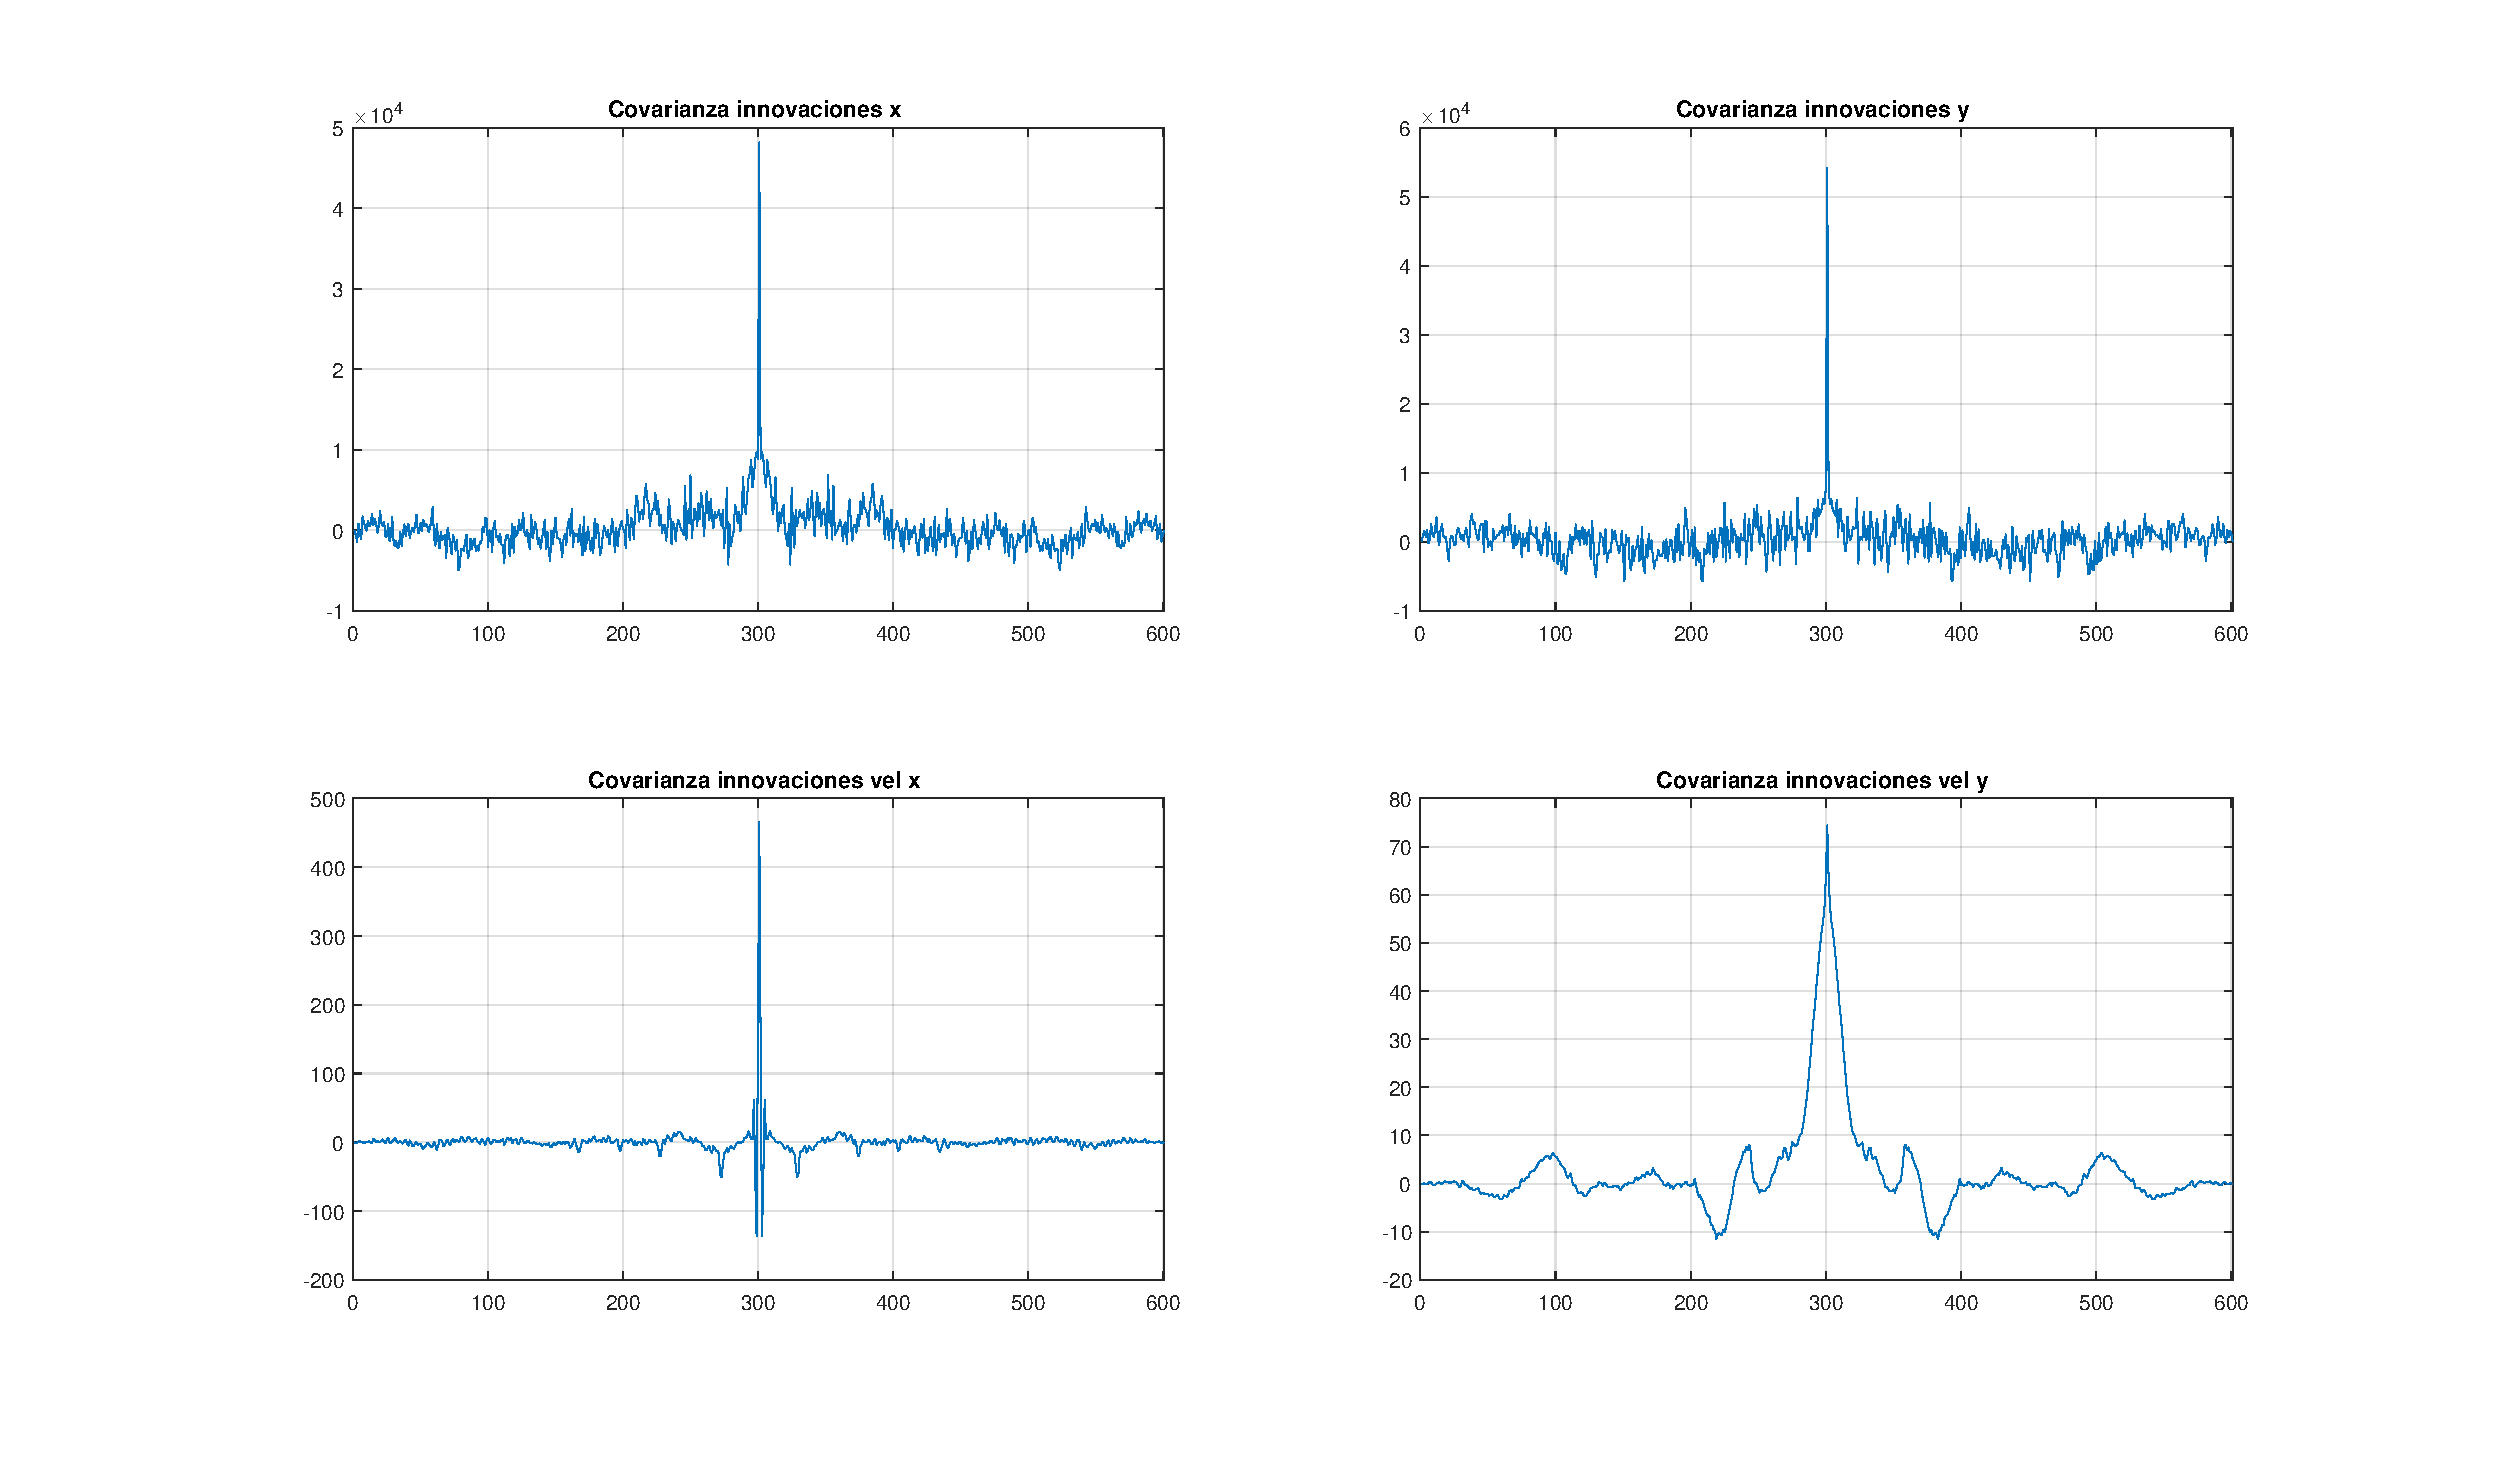
\includegraphics[width=0.9\textwidth,trim= 2cm 2cm 2cm 2cm]{graf_ej7_covinn.pdf}
\caption{Innovaciones de las posiciones y velocidades en $x^e$ e $y^e$.}
\label{fig:7covinn} 
\end{figure}
\vspace*{\fill}


\pagebreak


%\graficarPDFa{0 10cm 0 10cm}{graf_ej7_pos}{Posición y error de la misma en función del tiempo.}{fig:7pos}

\vspace*{\fill}
\begin{figure}[H]
\centering
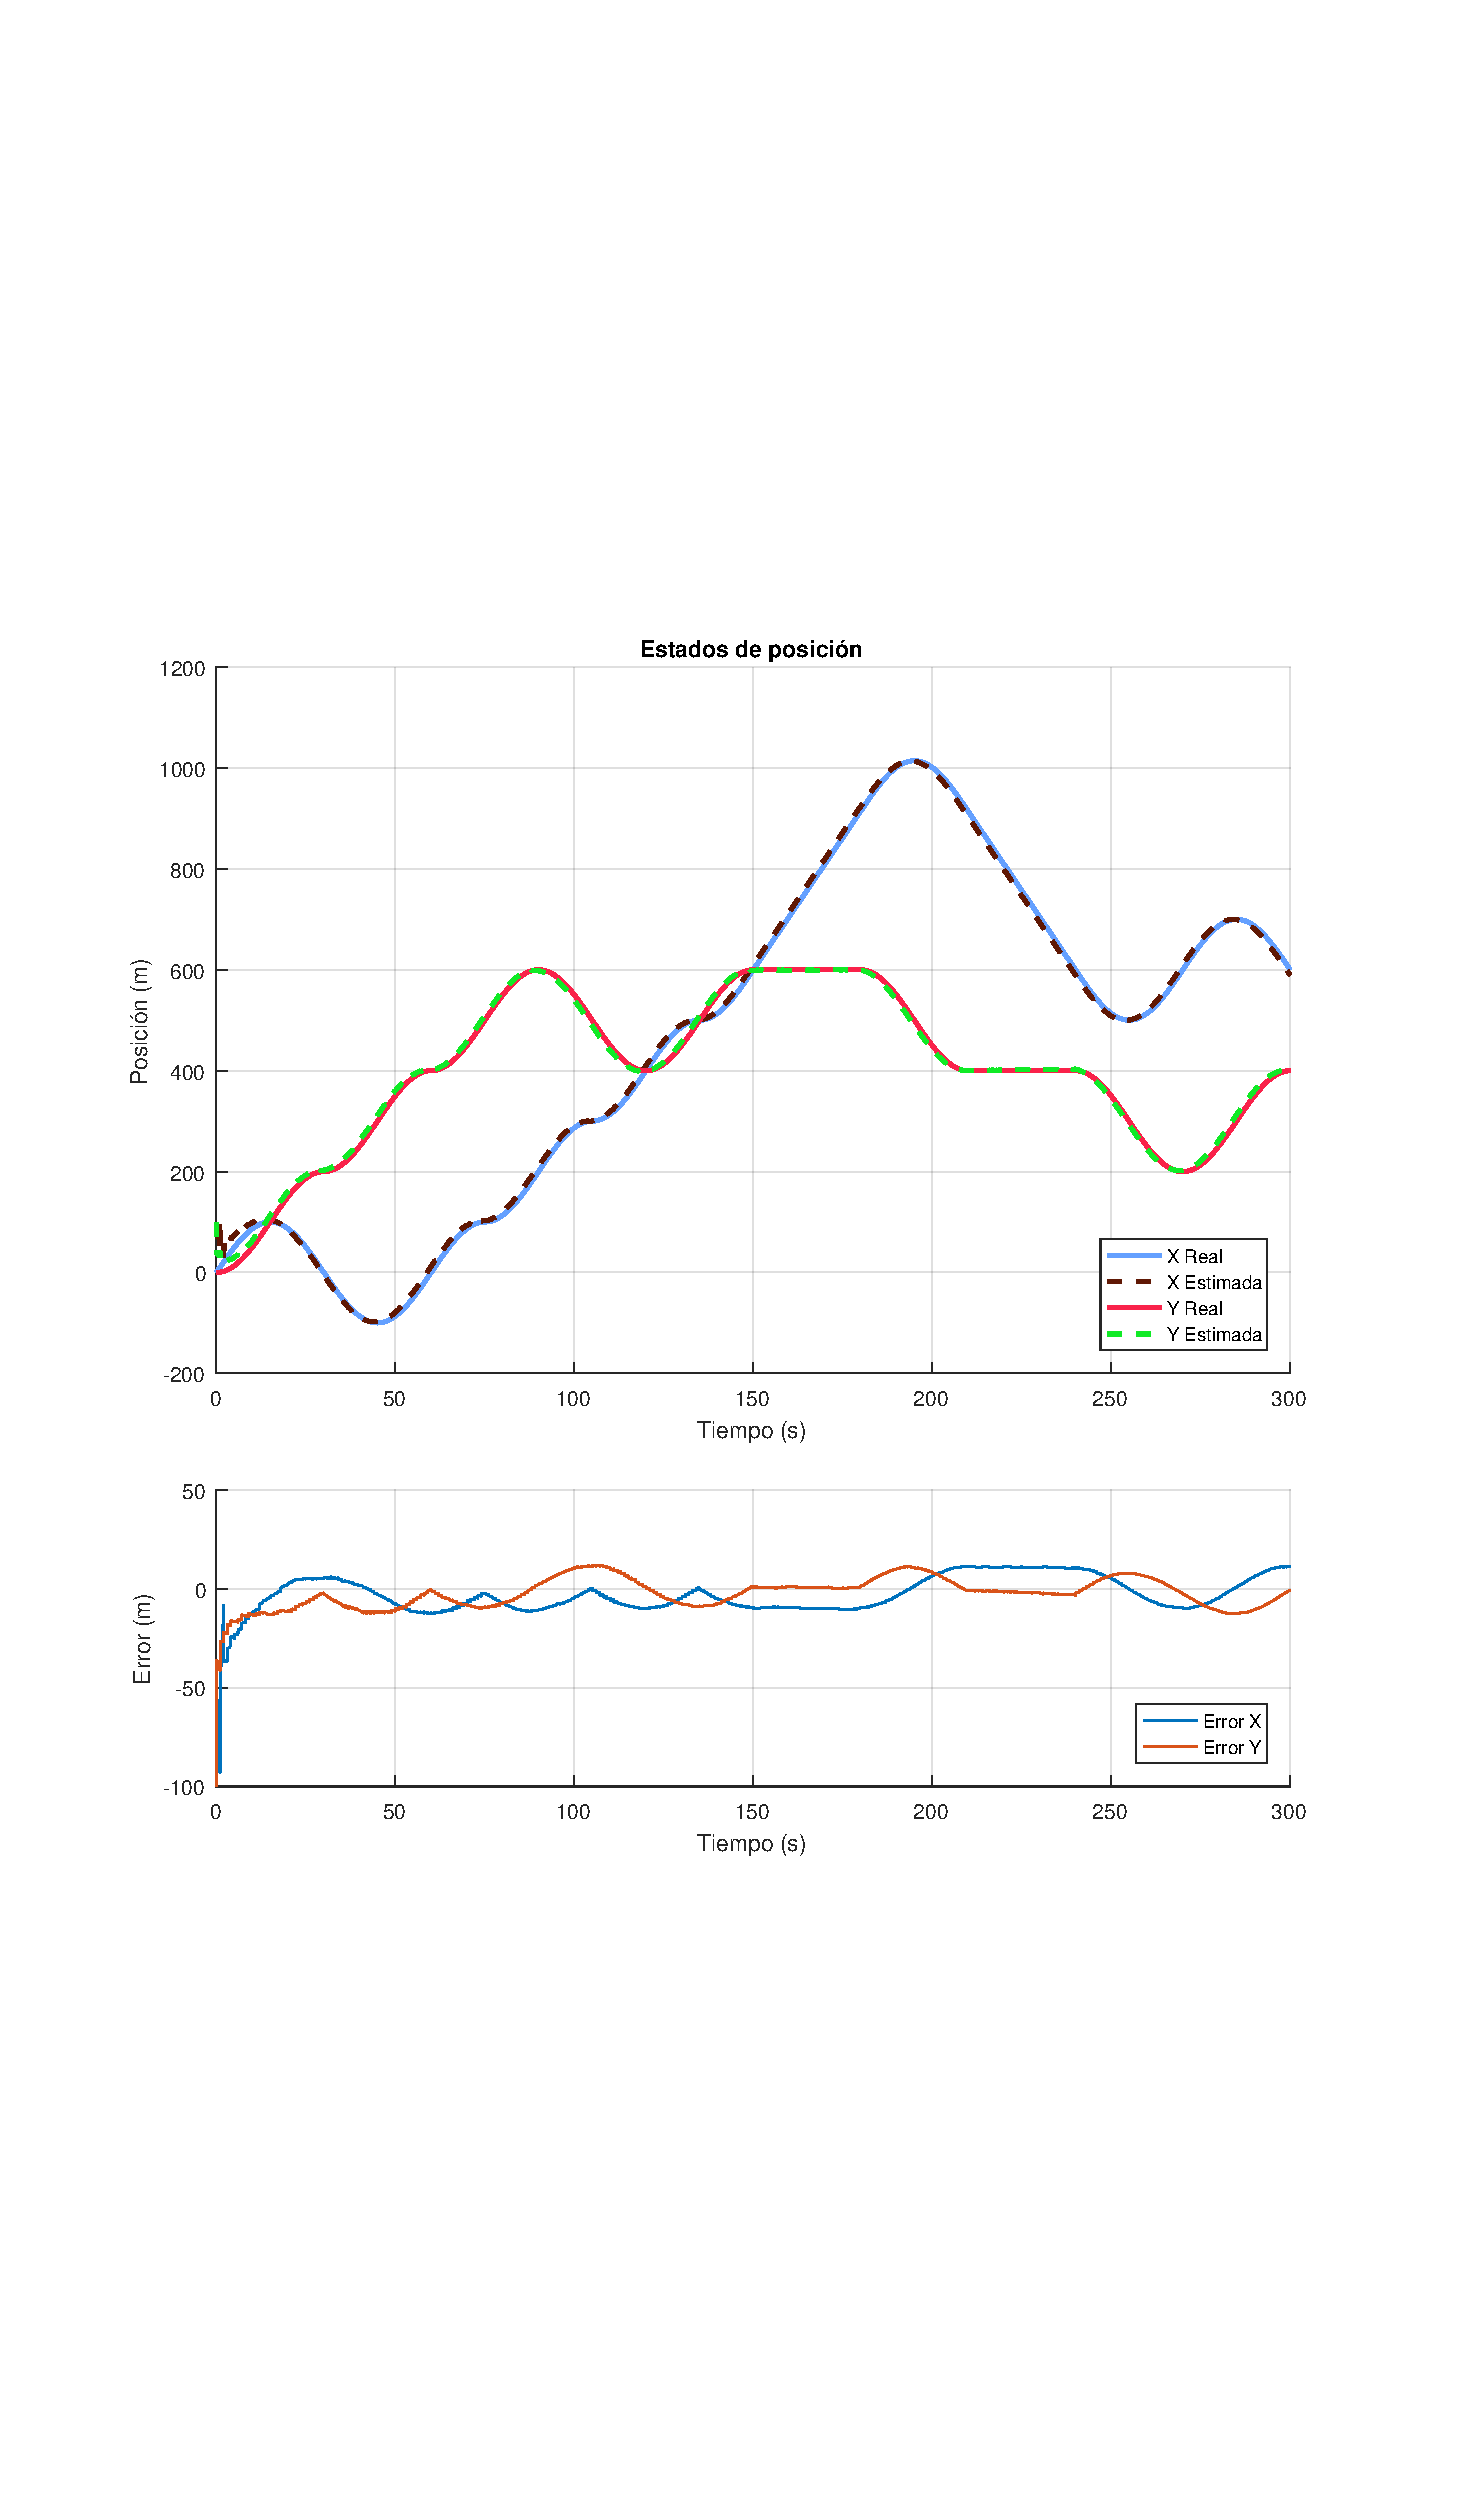
\includegraphics[scale=0.65, trim= 6cm 6cm 6cm 6cm]{graf_ej7_pos.pdf}
\caption{Posición y error en función del tiempo.}
\label{fig:7pos} 
\end{figure}
\vspace*{\fill}

\pagebreak

\graficarPDF{graf_ej7_theta}{Valores de los coeficientes de $C^e_b$ en el tiempo.}{fig:7theta}
\graficarPDF{graf_ej7_vel}{Velocidad real y estimada en función del tiempo.}{fig:7vel}
\graficarPDF{graf_ej7_sesgo}{Valores de los últimos \SI{100}{\s} del sesgo y su convergencia al valor real.}{fig:7sesgo}

%	\begin{equation*}
%		A\, \vect{x} = \begin{bmatrix} 
%			p_x + T\, v_x + (a^b_x - b_x)\frac{T^2}{2}\, c_{11} + (a^b_x - b_x)\frac{T^2}{2} \, c_{12} \\[0.3em]
%			p_y + T\, v_y + (a^b_x - b_x)\frac{T^2}{2}\, c_{21} + (a^b_x - b_x)\frac{T^2}{2} \, c_{22} \\[0.3em]
%			v_x + ac * c11 + ad * c12 \\[0.3em]
%			v_y + ac * c21 + ad * c22 \\[0.3em]
%			s1 * c11 + s2 * c12 \\[0.3em]
%			- s2 * c11 + s1 * c12 \\[0.3em]
%			s1 * c21 + s2 * c22 \\[0.3em]
%			- s2 * c21 + s1 * c22 \\[0.3em]
%			b_x \\[0.3em]
%			b_y \\[0.3em]
%		\end{bmatrix}
%	\end{equation*}



%		\begin{equation*}
%			Ad = \begin{bmatrix} 1& 0& T& 0&                 \frac{T^2(a_x - b_x)}{2}&                 \frac{T^2(a_y - b_y)}{2}&                                 0&                                 0&          -\frac{T^2c11}{2}&          -\frac{T^2c12}{2}\\[0.3em]
%			0& 1& 0& T&                                 0&                                 0&                 \frac{T^2(a_x - b_x)}{2}&                 \frac{T^2(a_y - b_y)}{2}&          -\frac{T^2c21}{2}&          -\frac{T^2c22}{2}\\[0.3em]
%		0& 0& 1& 0& T(a_x - b_x) - \frac{T^2\omega(a_y - b_y)}{2}& T(a_y - b_y) - \frac{T^2\omega(a_x - b_x)}{2}&                                 0&                                 0& \frac{c12\omega T^2}{2} - c11T& \frac{c11\omega T^2}{2} - c12T\\[0.3em]
%		0& 0& 0& 1&                                 0&                                 0& T(a_x - b_x) - \frac{T^2\omega(a_y - b_y)}{2}& T(a_y - b_y) - \frac{T^2\omega(a_x - b_x)}{2}& \frac{c22\omega T^2}{2} - c21T& \frac{c21\omega T^2}{2} - c22T\\[0.3em]
%           0& 0& 0& 0&                   1 - \frac{T^2\omega^2}{2}&                               T\omega&                                 0&                                 0&                     0&                     0\\[0.3em]
%           0& 0& 0& 0&                              -T\omega&                   1 - \frac{T^2\omega^2}{2}&                                 0&                                 0&                     0&                     0\\[0.3em]
%           0& 0& 0& 0&                                 0&                                 0&                   1 - \frac{T^2\omega^2}{2}&                               T\omega&                     0&                     0\\[0.3em]
%           0& 0& 0& 0&                                 0&                                 0&                              -T\omega&                   1 - \frac{T^2\omega^2}{2}&                     0&                     0\\[0.3em]
%           0& 0& 0& 0&                                 0&                                 0&                                 0&                                 0&                     1&                     0\\[0.3em]
%		0& 0& 0& 0&                                 0&                                 0&                                 0&                                 0&                     0&                     1\end{bmatrix}
%	\end{equation*}
%	En este caso se supone que la aceleración tiene un sesgo constante asociado. Es por tanto que la matriz $A(t)$ y el vector de estados se pueden reescribir como:
%			\begin{equation*}
%			A(t) = \begin{pmatrix}0&0&1&0&0&0&0&0&0&0\\[0.3em]0&0&0&1&0&0&0&0&0&0\\[0.3em]0&0&0&0&a^b_x - b_x&a^b_y - b_y&0&0&0&0\\[0.3em]0&0&0&0&0&0&a^b_x -b_x&a^b_y - b_y&0&0\\[0.3em]0&0&0&0&0&\omega^b&0&0&0&0\\[0.3em]0&0&0&0&-\omega^b&0&0&0&0&0\\[0.3em]0&0&0&0&0&0&0&\omega^b&0&0\\[0.3em]0&0&0&0&0&0&-\omega^b&0&0&0\\[0.3em]0&0&0&0&0&0&0&0&1&0\\[0.3em] 0&0&0&0&0&0&0&0&0&1\end{pmatrix} \qquad%
%				\vect{x}(t) = \begin{bmatrix} {p_x}(t) \\[0.3em] p_y(t) \\[0.3em] {v_x}(t) \\[0.3em] v_y(t) \\[0.3em] c_{11}(t) \\[0.3em] c_{12}(t) \\[0.3em] c_{21}(t) \\[0.3em] c_{22}(t) \\[0.3em] b_x \\[0.3em] b_y \end{bmatrix}
%			\end{equation*}
%	
%	
%		Se realiza el mismo proceso de discretización que se utilizó en el ejercicio \ref{sec:ej2}, salvo que donde aparecen las aceleraciones aparecen la diferencia de las mismas con sus sesgos. Luego, al realizar el producto $A\vect{x}$ se obtienen funciones con dependecia de producto de estados, siendo ellas alineales dificultando la estimación del filtro de Kalman. Para solucionarlo, se utiliza el algoritmo de Kalman extendido donde se sigue la dinámica que se linealiza entorno a los estados previos. En la implementación del algoritmo, cada ciclo genera la matriz $A_d = \frac{\partial{f_d}}{\partial \vect{x}}\left| _{\vect{x}=\vect{x}_{k-1/k-1}}\right. $ y a partir de la misma se realiza la predicción y/o corrección del filtro de Kalman tradicional.\\
%		\indent En la Figura \ref{fig:ej7} se puede ver la estimación de la trayectoria utilizando dicho algoritmo de estimación. Por medio de las Figuras \ref{fig:7covinn} y \ref{fig:7pos} puede verificarse los resultados del filtro. La Figura \ref{fig:7sesgo} muestra la convergencia de los valores del sesgo en los últimos \SI{100}{\s} de la trayectoria.
%		\Juan{Podríamos agregar un gráfico de los valores de $P$ de los sesgos para ver si va saltando o si se va achicando gradualmente}
%	
